\newpage

\section{Pianificazione}
La Pianificazione è un'attività essenziale per ottenere la massima efficacia ed efficienza nel lavoro richiesto dal progetto. Il team \textit{\gruppo} ha scelto di suddividere il carico di lavoro nei seguenti periodi:
\begin{itemize}
	\item \textbf{\AR};
	\item \textbf{\PA};
	\item \textbf{\PD};
	\item \textbf{\CO};
	\item \textbf{\VV}.
\end{itemize}
Per ognuno di questi periodi, vengono messe in evidenza, attraverso un \textit{\textbf{diagramma di Gantt\ped{G}}}, le principali attività richieste. Ogni attività, a sua volta, può essere suddivisa in una o più sotto-attività e fare riferimento ad una o più risorse. I diagrammi di Gantt permettono di rappresentare le varie dipendenze tra attività e sotto-attività, grazie all’uso di semplici frecce, e le relative risorse impiegate per ognuna di esse. La rappresentazione temporale delle attività nel diagramma di Gantt avviene mediante delle frecce direzionate verso il basso. In un diagramma di Gantt, inoltre, è possibile rappresentare delle \textit{milestone\ped{G}}, ovvero degli obiettivi da raggiungere, tramite dei rombi neri. Una milestone può essere:
\begin{itemize}
	\item \textbf{Esterna}, se coincide con le date di consegna dei documenti stabilite;
	\item \textbf{Interna}, se rappresenta un punto di revisione stabilito dal team.
\end{itemize}
Una milestone, quindi, coincide con la terminazione di un periodo, ed occorre fare attenzione a non causare dei ritardi su un'attività, poichè essi provocano lo slittamento temporale di tutte le attività ad essa collegate.

	\subsection{Suddivisione delle attività}
		\subsubsection{\AR}
		\textbf{Periodo}: dal 2016-12-02 al 2017-01-24.\\
		Il periodo inizia con la formazione del gruppo e termina con la consegna dei documenti richiesti per la \RR. Essa, infatti, richiede la produzione dei seguenti documenti:
		\begin{itemize}
			\item \textbf{\NdP}: primo documento da stilare, poiché definisce il modo in cui il team lavora e affronta ogni attività richiesta dal progetto. \MakeUppercase{è} responsabilità dell’\textit{\Amm}\ redigere questo documento, mentre i \textit{\Vers}\ avranno il compito di certificare che tutte le norme stilate siano realmente osservate durante le varie attività;
			\item \textbf{\SdF}: all'interno di questo documento viene raccolta un'analisi per ognuno dei capitolati proposti, la quale mette in evidenza il dominio tecnologico e quello applicativo, e valuta gli aspetti positivi e negativi. Lo \SdF\ è un’attività molto importante, perché consente di scegliere il progetto più adatto per lo specifico gruppo, basandosi su una o più considerazioni motivate e ponderate;
			\item \textbf{\AdR}: documento di responsabilità degli \textit{\Anas}, che contiene un’analisi molto più approfondita del capitolato scelto in seguito allo \SdF;
			\item \textbf{\PdP}: documento stilato dal \textit{\RdP}, che individua tutte le attività necessarie allo svolgimento del progetto e le assegna alle risorse disponibili. Il punto importante sul quale occorre porre maggiore attenzione è come distribuire il carico di lavoro in maniera uniforme. Questo documento ha un'alta priorità, poiché vincola tutte le attività che sono e saranno svolte dal team nel corso del progetto;
			\item \textbf{\PdQ}: documento di responsabilità del \textit{\Ver}, il quale definisce le metodologie di verifica adottate, al fine di aumentare la qualità del prodotto richiesto;
			\item \textbf{\G}: questo documento viene scritto in maniera incrementale da ogni redattore di un documento. Contiene la spiegazione dei termini tecnici utilizzati nei vari documenti, in modo da consentire una facile comprensione priva di ambiguità, qualunque sia il lettore del documento;
			\item \textbf{\LdP}: documento che presenta il gruppo e la sua proposta di partecipazione alla gara d’appalto per il capitolato scelto.
		\end{itemize}
		I ruoli maggiormente interessati in questa fase, per la produzione dei documenti citati, sono: \textit{\Amm}, \textit{\Res}, \textit{\Ana}\ e \textit{\Ver}.
		
		%qua inizia tabella con gantt
		%ho usato smartsheet, un'app web
		\begin{figure}[H]
			\centering
			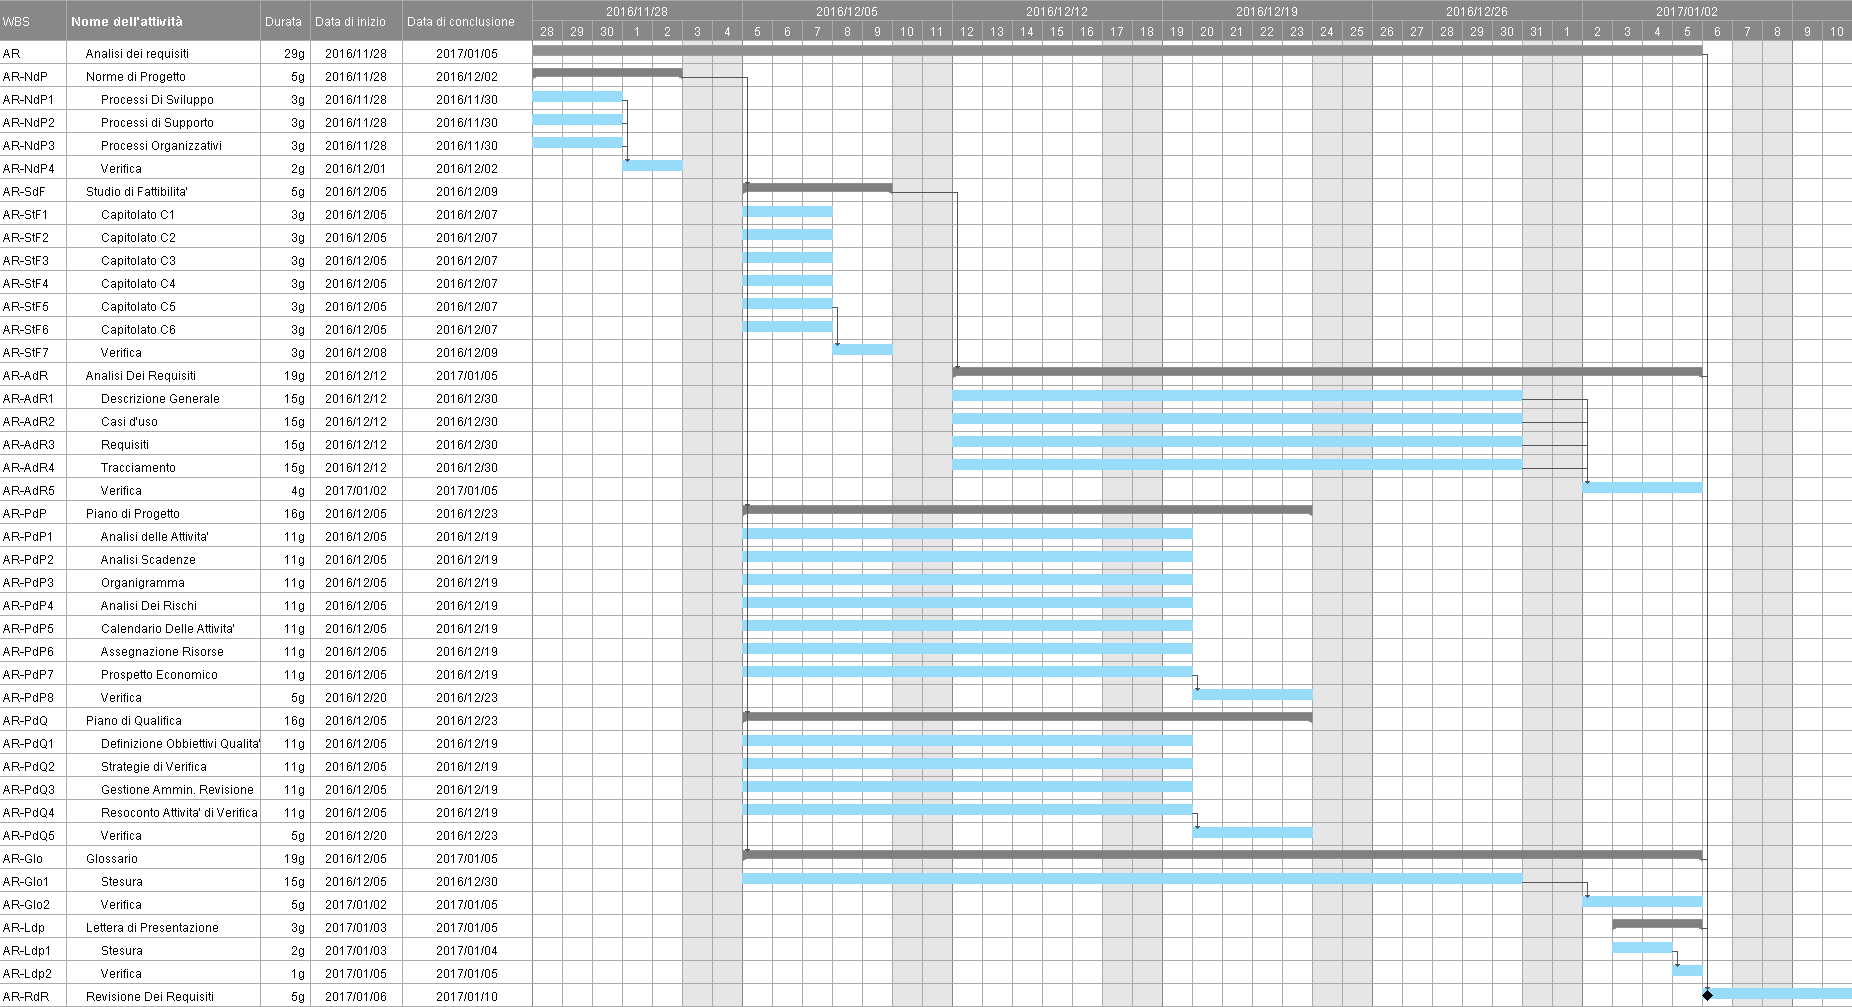
\includegraphics[angle=90,scale=0.37]{img/ganttnetbreak1.png}
			\caption{Diagramma di Gantt relativo al periodo di Analisi dei Requisiti}
		\end{figure}
		%qua finisce tabella con gantt
		
		\subsubsection{\ARD}
		\textbf{Periodo}: dal 2017-01-25 al 2017-02-24.\\
		L'inizio di tale periodo coincide con la consegna dei documenti per la \RR\ e ha la durata di circa un mese, antecedentemente rispetto al periodo preposto alla \PA. Durante questo periodo, il gruppo può analizzare la valutazione emersa dalla \RR\ ed effettuare le opportune correzioni. In questo periodo, inoltre, l'obiettivo è consolidare i requisiti individuati e procedere con la correzione di tutti i documenti inerenti alla consegna. La scadenza segnalata è una scadenza puramente interna al gruppo \textit{\gruppo}.
		
		\begin{figure}[H]
			\centering
			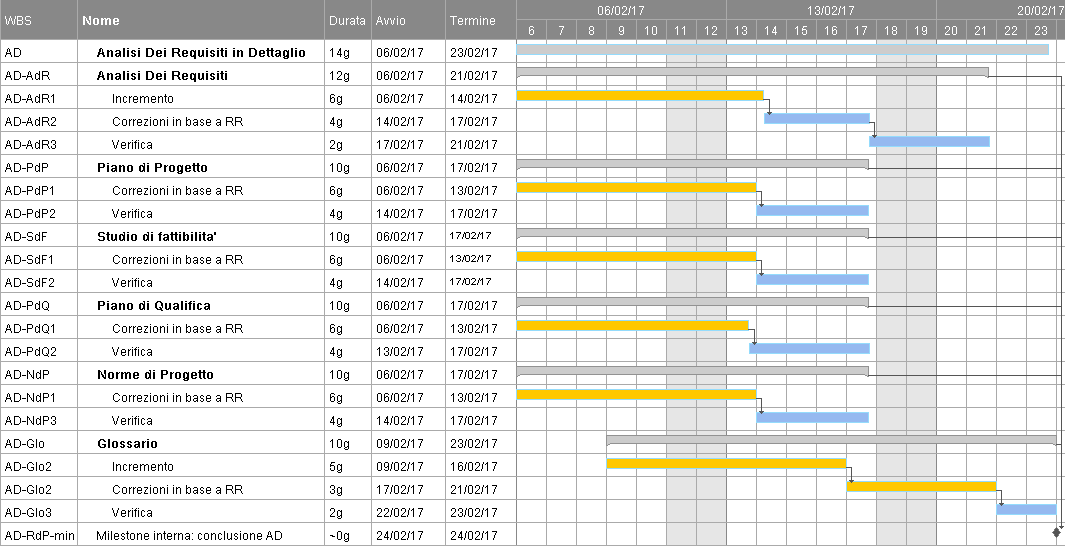
\includegraphics[scale=0.3]{img/ganttnetbreak2.png}
			\caption{Diagramma di Gantt relativo al periodo di Analisi dei Requisiti Dettagliata}
		\end{figure}
		
		
		\subsubsection{\PA}
		\textbf{Periodo}: dal 2017-02-25 al 2017-03-13.\\
		Il periodo di \PA\ inizia immediatamente dopo l'\AR\ e termina con la milestone prestabilita di \RPMin. Nell'arco di questo periodo è necessario effettuare la progettazione ad alto livello del sistema. Inoltre, si richiede di svolgere le seguenti attività:
		\begin{itemize}
			\item \textit{\ST}: documento che interessa prevalentemente il \textit{\Prog}\ del team. In esso vengono specificate:
			\begin{itemize}
				\item Scelte progettuali di alto livello prese;
				\item Design pattern scelti per la realizzazione del prodotto;
				\item Architettura generale del software.
			\end{itemize}
			\item Migliorare i documenti \NdP, \PdP, \PdQ\ e \G;
			\item Verificare e approvare tutti i documenti modificati.
		\end{itemize}
		I ruoli maggiormente interessati in questo periodo sono: \textit{\Amm}, \textit{\Res}, \textit{\Prog} e \textit{\Ver}.
		
		%qua inizia tabella con gantt
		%ho usato smartsheet, un'app web
		\begin{figure}[H]
			\centering
			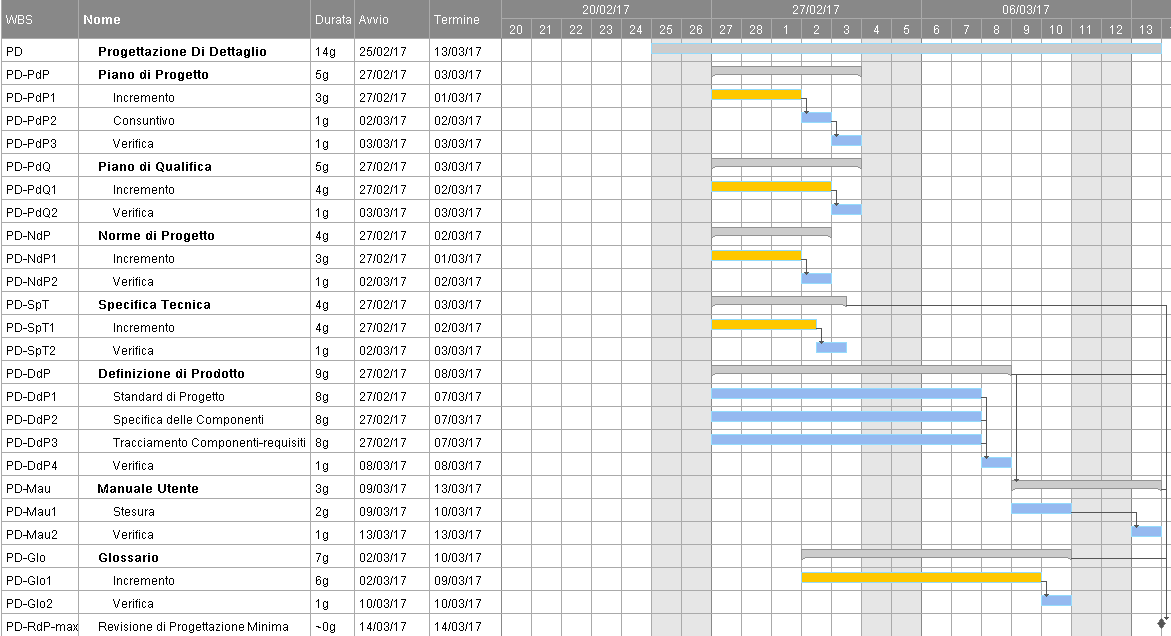
\includegraphics[scale=0.4]{img/ganttnetbreak3.png}
			\caption{Diagramma di Gantt relativo al periodo di Progettazione Architetturale}
		\end{figure}

		%qua finisce tabella con gantt
	
		\subsubsection{\PD}
		\textbf{Periodo}: dal 2017-03-14 al 2017-03-24.\\
		Il periodo di \PD\ inizia dopo quello di \PA\ e, in un'ottica di una progettazione di minimo, viene incorporata con la consegna dei documenti previsiti dalla \RQ. Questo periodo prevede la stesura dettagliata dell’intero sistema, specificando approfonditamente il comportamento e l’interazione tra i vari componenti. La scadenza individuata per questo periodo è puramente interna, dal momento che come è stato menzionato in precedenza, il gruppo NetBreak affronterà la progettazione con un livello di dettaglio intermedio (e non in una progettazione di massima per la scadenza della \RP).
		La Progettazione Architetturale Dettagliata prevede lo svolgimento delle seguenti attività:
		\begin{itemize}
			\item \textit{\DDP}: documento di responsabilità del \textit{\Prog}, il quale ha il compito di descrivere il comportamento	e le interazioni tra i vari componenti del sistema, basandosi sul documento di \ST;
			\item  Migliorare i documenti \NdP, \PdP, \PdQ, \ST\ e \G;
			\item Verificare e approvare tutti i documenti modificati.
		\end{itemize}
		I ruoli maggiormente interessati in questo periodo sono: \textit{\Amm}, \textit{\Res}, \textit{\Prog}\ e \textit{\Ver}.
		
		%qua inizia tabella con gantt
		%ho usato smartsheet, un'app web
		\begin{figure}[H]
			\centering
			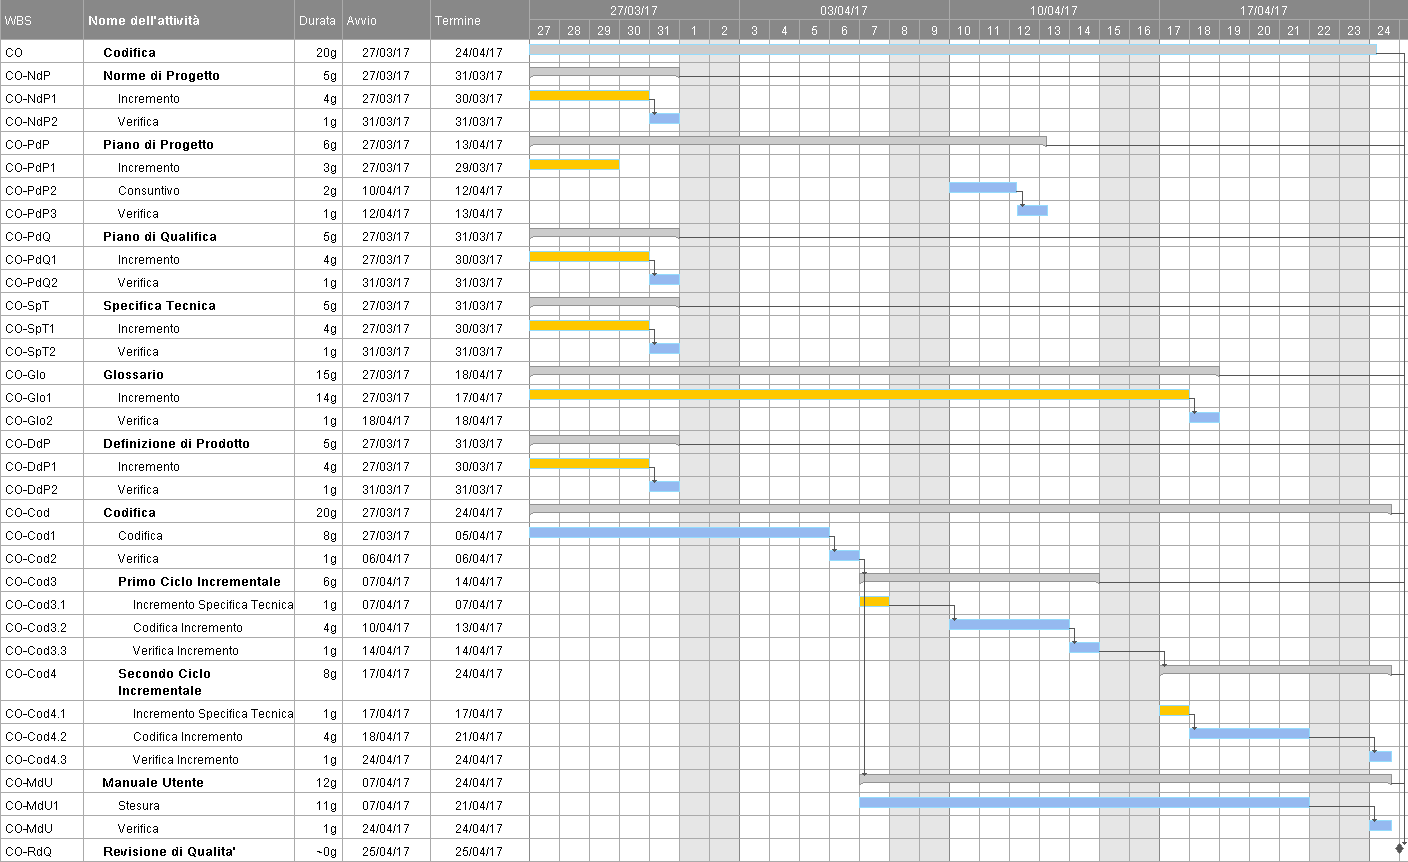
\includegraphics[scale=0.43]{img/ganttnetbreak4.png}
			\caption{Diagramma di Gantt relativo al periodo di Progettazione Architetturale Dettagliata}
		\end{figure}
		%qua finisce tabella con gantt
		
		\subsubsection{\CO}
		\textbf{Periodo}: dal 2017-03-25 al 2017-04-18.\\
		Il periodo di \CO\ è successivo alla \PD\ e si conclude con la consegna del prodotto per la \RQ. Questo periodo ha l'obiettivo di fornire un prodotto qualificato, grazie allo svolgimento delle seguenti attività:
		\begin{itemize}
			\item \textbf{Codifica}: i \textit{\Progrs}\ hanno il compito di sviluppare il codice del prodotto software progettato nelle precedenti attività e descritto nel documento \DDP. L’attività di Codifica prevede due cicli incrementali per: il miglioramento
			di parti del sistema già esistenti e funzionanti, e l’aggiunta di nuove funzionalità al sistema stesso.
			Ogni incremento prevede tre attività:
			\begin{itemize}
				\item Progettazione dell’incremento da parte dei \textit{\Progs};
				\item Codifica da parte dei \textit{\Progrs} dell’incremento progettato;
				\item Verifica dell’incremento effettuato.
			\end{itemize}
			\item \textit{\MU}: documento che descrive le linee guida per il corretto utilizzo del prodotto. Esso è destinato all’utilizzatore finale/cliente;
			\item  Migliorare i documenti \NdP, \PdP, \PdQ\ e \G;
			\item Verificare e approvare tutti i documenti modificati.
		\end{itemize}
		I ruoli maggiormente interessati in questo periodo sono: \textit{\Amm}, \textit{\Res}, \textit{\Prog}, \textit{\Progr}\ e \textit{\Ver}.
		
		%qua inizia tabella con gantt
		%ho usato smartsheet, un'app web
		\begin{figure}[H]
			\centering
			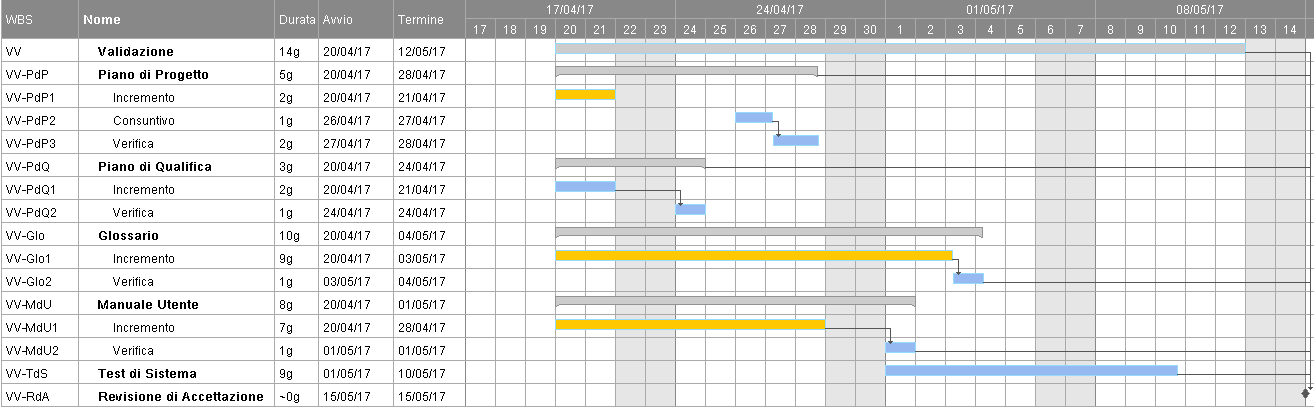
\includegraphics[scale=0.40]{img/ganttnetbreak5.png}
			\caption{Diagramma di Gantt relativo al periodo di Codifica}
		\end{figure}
		%qua finisce tabella con gantt
		
		\subsubsection{\VV}
		\textbf{Periodo}: dal 2017-04-19 al 2017-05-15.\\
		Il periodo di \VV\ inizia dopo quello di \CO\ e termina con la consegna del prodotto finale alla \RA. Questo periodo ha lo scopo di effettuare tutti i test necessari a garantire che il prodotto sia conforme alla attese e soddisfi tutti i requisiti concordati e descritti in \AdR. Le attività previste sono:
		\begin{itemize}
			\item Effettuare i test di sistema;
			\item Migliorare i documenti \NdP, \PdP, \PdQ, \G\ e \MU;
			\item Verificare e approvare tutti i documenti modificati.
		\end{itemize}
			I ruoli maggiormente interessati in questo periodo sono: \textit{\Res}, \textit{\Prog}\ e \textit{\Ver}.
			
		%qua inizia tabella con gantt
		%ho usato smartsheet, un'app web
		\begin{figure}[H]
			\centering
			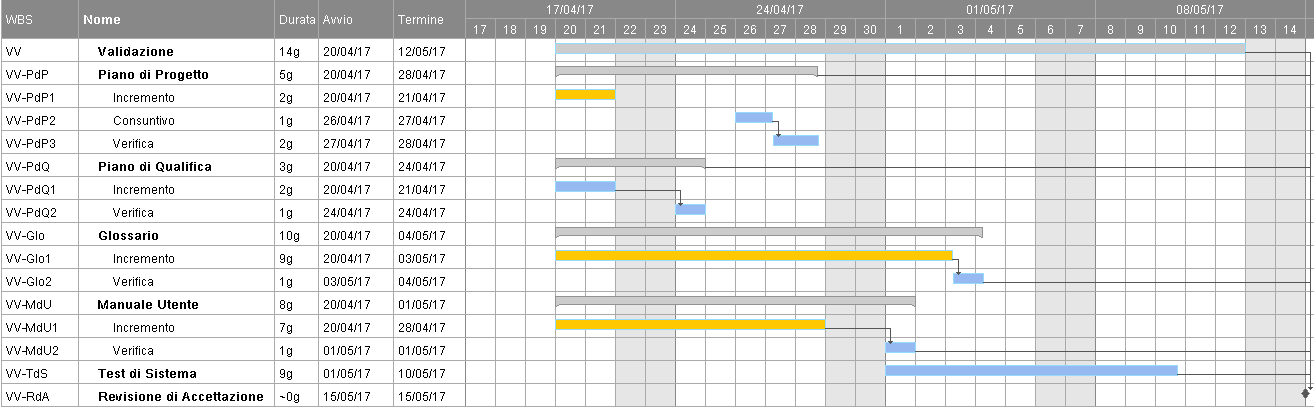
\includegraphics[scale=0.34]{img/ganttnetbreak6.png}
			\caption{Diagramma di Gantt relativo al periodo di Verifica e Validazione}
		\end{figure}
		%qua finisce tabella con gantt